\documentclass{article}
\usepackage[utf8]{inputenc}
\usepackage{geometry}
\usepackage{float}
\usepackage[backend=bibtex, style=numeric]{biblatex}
\usepackage{hyperref}
\hypersetup{
    colorlinks=true,
    linkcolor=blue,     
    urlcolor=magenta,
    pdfpagemode=FullScreen,
}
 \geometry{
 a4paper,
 total={170mm,257mm},
 left=20mm,
 top=20mm,
 }
 \usepackage{graphicx}
 \usepackage{titling}

 \title{Exploring Variants of the Art Gallery Problem
}
\author{Pradyumnan R}
\date{August 2024}
 
 \usepackage{fancyhdr}
\fancypagestyle{plain}{%  the preset of fancyhdr 
    \fancyhf{} % clear all header and footer fields
    % \fancyfoot[R]{
\includegraphics[width=2cm]{IITM_Logo.png}}
    \fancyfoot[L]{\thedate}
    \fancyhead[L]{ED5310 - Algorithms in Computational Geometry}
    \fancyhead[R]{\theauthor}
}
\makeatletter
\def\@maketitle{%
  \newpage
  \null
  \vskip 1em%
  \begin{center}%
  \let \footnote \thanks
    {\LARGE \@title \par}%
    \vskip 1em%
    %{\large \@date}%
  \end{center}%
  \par
  \vskip 1em}
\makeatother

\usepackage{lipsum}  
\usepackage{cmbright}

\addbibresource{refs.bib}

\begin{document}

\maketitle

\noindent\begin{tabular}{@{}ll}
    By \theauthor \\
\end{tabular}

\section*{Introduction}
In this report, we shall explore a few variants of the art gallery problem. The report systematically describes all variants by giving an overview of the variants' problem statement, the underlying assumptions, the current state of the problem and sometimes even a solution, if one exists. \\

\noindent Some relevant definitions are discussed below : -

\begin{itemize}

	\item A simple polygon $P = \left( v_0, v_1, \cdots, v_n \right)$ is a closed plane figure whose boundary $bd(P)$ is composed of straight line edges $\left( v_i, v_{i+1} \right), \: i = 0, 1, \cdots, n - 1, \: v_0 = v_n$, and where no two non-consecutive edges intersect. When the edges are traversed in a counterclockwise sense, the interior is always to the left.
	
	\item Two points $p$ and $q$ are said to be visible from each other if the line segment $pq$ connecting them lies completely in $P$. 
	
	\item A point $p$ of $P$ is said to be visible from an edge $\left( u, v \right)$ if there exists a point $q$ on $\left(u, v \right)$ such that $p$ and $q$ are visible.
	
	\item For any point $v$ of $P$, the $v$-cover is the locus of the points of $P$ that are visible from $v$. The $(u, v)$-cover is defined similarly.
	
	\item A ploygon is called \textbf{star-shaped} if there exists a point $v$ in $P$ such that the $v$-cover is the polygon $P$ itself.
	
	\item The \textbf{kernel} of a polygon $P$ is the region in $P$ such that for any point $q$ in $P$, $q$ is visible from any point in this region.
	
\end{itemize}

\section{Edge Guard Problem}

For this particular problem, I have referred to the paper published in \textit{IEEE Transactions on Information Theory, Vol. IT-32, No. 2, March 1986} titled \textit{Computational Complexity of Art Gallery Problems} by D. T. Lee and Arthur K. Lin \cite{lee1986computational}. \\

\noindent \textbf{Problem Statement :} What are the minimum number of guards that can each traverse along a particular edge that are required such that every point in a polygon $P$ can be seen by the guards. More formally, what are minimum number of edges $(u, v)$ whose $(u, v)$-cover is the entire polygon $P$. \\

\noindent \textbf{Assumptions : -}

\begin{enumerate}

	\item Every guard can view $360 ^ \circ$ around them at every instant
	
	\item Every guard has an infinite range of vision
	
	 \item Every guard can move strictly on a particular edge of the polygon that is predetermined
	
	\item The polygon is simply connected \textit{i.e.,} has no holes
	
	\item The polygon is strictly is 2 dimensional
	
\end{enumerate}

\noindent \textbf{State of the problem :} The problem has been shown in \cite{lee1986computational} to be NP-hard.

\section{Two Guards Problem}

For this particular problem, I have referred to the conference paper from the \textit{Proceedings of the ninth annual symposium on Computational Geometry} titled \textit{An optimal algorithm for the two-guard problem} by Paul.J.Heffernan \cite{heffernan1993optimal}. \\

\noindent \textbf{Problem Statement :} Given a simple polygon $P$ with vertices $s$ and $t$, the \textit{straight walk} problem asks whether we can move two points monotonically from $s$ to $t$, one clockwise and one counterclockwise, such that the points are covisible. In the \textit{counter-walk problem}, both points move clockwise, one from $s$ to $t$ and the other from $t$ to $s$. \\ 

\noindent \textbf{Assumptions : -}

\begin{enumerate}

	\item Every guard can view $360 ^ \circ$ around them at every instant
	
	\item Every guard has an infinite range of vision
	
	 \item Every guard can move freely on any edge of the polygon in a continuous fashion
	
	\item The polygon is simply connected \textit{i.e.,} has no holes
	
	\item The polygon is strictly is 2 dimensional
	
\end{enumerate}

\noindent \textbf{State of the problem :} Heffernan has provided $\Theta(n)$ algorithms for both the straight walk and the counter walk problems. This is an improvement over the $O(nlogn)$ algorithms provided by Icking and Kline in \cite{icking1992two}.


\section{Conflict-Free Chromatic Art Gallery Problem}

For this particular problem, I have referred to the paper from the \textit{Algorithmca} journal titled \textit{Conflict-Free Chromatic Art Gallery Coverage} by Bartschi and Suri \cite{bartschi2014conflict}. \\

\noindent \textbf{Problem Statement :} We consider a polygon $P$ and guards who are each assigned one of $k$-distinct colors. A placement of such guards is conflict-free if each point of the polygon is seen by some guard whose color appears exactly once among the guards visible to that point. What is the smallest number of colors $k(n)$ to ensure a conflict-free covering of all $n$-vertex polygons. \\ 

\noindent \textbf{Assumptions : -}

\begin{enumerate}

	\item Every guard can view $360 ^ \circ$ around them at every instant
	
	\item Every guard has an infinite range of vision
	
	 \item Distinct guards are placed at distinct vertices of the polygon
	
	\item The polygon is simply connected \textit{i.e.,} has no holes
	
	\item The polygon is strictly is 2 dimensional
	
\end{enumerate}

\noindent \textbf{State of the problem :} Barthschi and Suri have shown in \cite{bartschi2014conflict} that for orthogonal and monotone polygons $k(n)$ can be found in $O(logn)$ and for arbitrary simple polygons, $k(n)$ can be found in $O(log^2n)$.

\begin{figure}[H]
  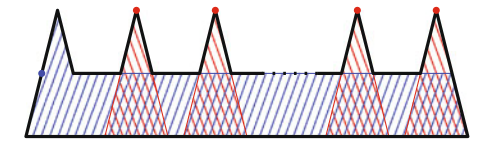
\includegraphics[scale=0.7]{Chromatic.png}
  \centering
  \caption{\textbf{Chromatic Version of the Art Gallery Problem}}
  \label{img:chromatic}
\end{figure}

\section{Half Guard}

For this particular problem, I have referred to the paper from the \textit{42nd IARCS Annual Conference on Foundations of Software Technology and Theoretical Computer Science (FSTTCS 2022)} titled \textit{Half-Guarding Weakly-Visible Polygons and Terrains} by Duraisamy et al. \cite{duraisamy2022half}. \\

\noindent \textbf{Problem Statement :} We consider a polygon $P$ and are required to find the minimum number of guards required to guard $P$. For the \textit{terrain guarding} problem, we consider a terrain and find the minimum number of guards required to view every point on the terrain. For both these problems, we have the additional constraing that the guards are all \textit{half guards}. \\ 

\noindent \textbf{Assumptions : -}

\begin{enumerate}

	\item Every guard can view exactly $180 ^ \circ$ around them at every instant
	
	\item The guards can be oriented in any direction
	
	\item Every guard has an infinite range of vision
	
	 \item Distinct guards are placed at distinct vertices of the polygon
	
	\item The polygon is simply connected \textit{i.e.,} has no holes
	
	\item The polygon is strictly is 2 dimensional
	
\end{enumerate}

\noindent \textbf{State of the problem :} Duraisamy et al. have shown in \cite{duraisamy2022half} that the half guard problem is NP-hard for weakly visible polygons. Interestingly for terrains, the problem is highly dependent on the orientation of the guards and accordingly becomes very easy (polynomial time) or very difficult (NP-hard).

\begin{figure}[H]
  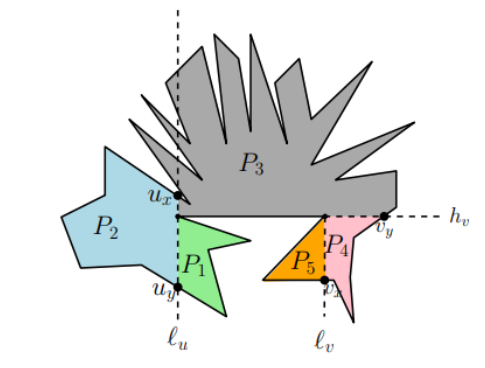
\includegraphics[scale=0.5]{Half.png}
  \centering
  \caption{\textbf{Half Guard Variant of the Art Gallery Problem}}
  \label{img:half}
\end{figure}

\section{k-Consecutive Guards Fortress Problem}

For this particular problem, I have referred to the paper from the \textit{Vol.72, Journal of Geometry, 2001} titled \textit{A generalized fortress problem using $k$-consecutive vertex guards} by S.M.Yiu \cite{yiu2001generalized}. \\

\noindent \textbf{Problem Statement :} We consider a polygon $P$ and are required to find the minimum number of guards that can guard the entire exterior of the $P$ out of which $k$ of them are located on an $k$-consecutive vertices.\\ 

\noindent \textbf{Assumptions : -}

\begin{enumerate}

	\item Every guard can view exactly $360 ^ \circ$ around them at every instant
	
	\item Every guard has an infinite range of vision
	
	 \item Distinct guards are placed at distinct vertices of the polygon
	
	\item The polygon is simply connected \textit{i.e.,} has no holes
	
	\item The polygon is strictly is 2 dimensional
	
	\item $k$ of the guards have to be placed at continous vertices
	
\end{enumerate}

\noindent \textbf{State of the problem :} Yiu showed in \cite{yiu2001generalized} that $\left \lceil n / (k+1) \right \rceil$ $k$-consecutive guards are sometimes necessary and always sufficient to cover the entire exterior of $P$.

\clearpage

\printbibliography

\end{document}
